\documentclass[12pt,a4paper,twoside]{article}

\usepackage{mystyle}

\def\footnoteDergachev{A.\,A.~Dergachev,~dergachev88@yandex.ru}
\def\footnoteEfimov{O.\,V.~Efimov,~efimovov@yandex.ru}
\def\footnoteSmetanina{E.\,O.~Smetanina,~jannes-2002@yandex.ru}

\begin{document}

	\thispagestyle{empty}

    % УДК: http://teacode.com/online/udc/
    % 519.633: Дифференциальные уравнения второго порядка параболического и гиперболического типов
    % 519.684: Программирование для специализированных вычислительных машин
    % 519.688: Программы и алгоритмы для решения отдельных задач на вычислительных машинах
    \noindent УДК 519.633:519.684:519.688

    \noindent \textbf{ОБЗОР И СРАВНИТЕЛЬНЫЙ АНАЛИЗ ПАРАЛЛЕЛЬНЫХ ЧИСЛЕННЫХ АЛГОРИТМОВ РЕШЕНИЯ НЕЛИНЕЙНОГО УРАВНЕНИЯ ШРЁДИНГЕРА}

	\vspace{1em}

    \noindent \copyright \quad 2010 г. \quad \textbf{
    	А.\,А.~Дергачёв\footnote[1]{\footnoteDergachev},
    	О.\,В.~Ефимов\footnote[2]{\footnoteEfimov},
    	Е.\,О.~Сметанина\footnote[3]{\footnoteSmetanina}
   }

	\vspace{0.5em}

    \noindent Международный учебно-научный лазерный центр МГУ имени М.В. Ломоносова \\
    119991, ГСП-1, Москва, Ленинские горы, 1, стр. 62.

	\vspace{-3em}

    \begin{abstract}
        \noindent Рассматриваются параллельные численные методы решения нелинейного уравнения квазиоптики на основе разностных схем и быстрого преобразования Фурье.
        Приводятся результаты исследования производительности рассматриваемых методов на суперкомпьютере СКИФ <<Чебышёв>> и кластере IBM BlueGene/P,
        установленных в~Московском государственном университете имени М.\,В. Ломоносова.
        Статья подготовлена по результатам обучения по специальной программе <<Суперкомпьютерные технологии>> и собственных исследований в рамках научной работы.
        
        \vspace{1em}
        
        \noindent Ключевые слова: параллельные алгоритмы, нелинейное уравнение Шрёдингера,
        эффективность распараллеливания, метод прогонки, быстрое преобразование Фурье.
        
        \vspace{1em}
        
	    \noindent \textbf{REVIEW AND COMPARATIVE ANALYSIS OF PARALLEL NUMERICAL ALGORITHMS FOR NONLINEAR SCHRODINGER EQUATION SOLVING}
		
		\vspace{1em}
		
	    \noindent \textbf{A.\,A.~Dergachev\footnotemark[1],
	    	O.\,V.~Efimov\footnotemark[2],
	    	E.\,O.~Smetanina\footnotemark[3]
	    }
		
        \vspace{1em}
 		
        \noindent Рассматриваются параллельные численные методы решения нелинейного уравнения квазиоптики на основе разностных схем и быстрого преобразования Фурье.
        Приводятся результаты исследования производительности рассматриваемых методов на суперкомпьютере СКИФ <<Чебышёв>> и кластере IBM BlueGene/P,
        установленных в~Московском государственном университете имени М.\,В. Ломоносова.
        Статья подготовлена по результатам обучения по специальной программе <<Суперкомпьютерные технологии>> и собственных исследований в рамках научной работы.
        
        \vspace{1em}
        
        \noindent Keywords: parallel algorithms, nonlinear Schrodinger equation,
        parallelization efficiency, sweep method, fast Fourier transform.
    \end{abstract}

    %\hrule

    \vspace{0.5em}
\noindent \textbf{1. Введение и постановка задачи.}
\vspace{0.5em}

Нелинейное уравнение Шрёдингера играет существенную роль во многих областях физики, а также химии, экономики и иных наук.
Это уравнение на комплексную функцию $A(\vec{r},t)$ имеет вид:

\begin{equation}\label{NonlinearShredinger}
    \alpha i \dfrac{\partial A}{\partial t} = \beta \dfrac{\partial^2 A}{\partial x^2} + \gamma \left|A\right|^2 A
\end{equation}

Такое название присвоено уравнению (\ref{NonlinearShredinger}) потому, что его линейная часть совпадает с уравнением Шрёдингера.
В оптических приложениях чаще используется наименование <<нелинейное уравнение квазиоптики>>.

В нелинейной оптике это уравнение описывает самофокусировку  светового пучка в среде с кубической нелинейностью.
При описании распространения мощных коротких лазерных импульсов в диспергирующих средах
нелинейное уравнение для медленно меняющейся комплексной огибающей светового поля дополняют членами,
учитывающими дисперсию высших порядков, нелинейность отклика самоиндуцированной плазмы, потери на ионизацию и поглощение лазерного излучения в веществе \cite{KandidovShlenovKosarevaReview2009}.

В теории лазеров оптического диапазона с помощью нелинейного уравнения квазиоптики изучается усиление излучения, поиск собственных частот и типов колебаний поля в резонаторе.
Для исследования динамики усиленного спонтанного излучения в рентгеновском лазере используется квазиоптическое уравнение для поперечной корреляционной функции поля излучения \cite{LadaginStarikov1998}.

Распространение лазерных импульсов в оптических волноводах также описывается нелинейным уравнением квазиоптики для комплексной огибающей светового поля,
частными решениями которого являются темные (в области нормальной дисперсии групповых скоростей) и светлые (в области аномальной дисперсии групповых скоростей) солитоны \cite{Agrawal2001,Mahankov1983,VitkovskiyFedoruk2008}.

В физике сверхнизких температур нелинейное уравнение Шрёдингера используется для описания поведения неидеального бозе-газа со слабым взаимодействием между частицами \cite{Kadomcev1997}.
В работе \cite{Belyaeva2005} обращается внимание на математическую аналогию между теорией солитонных волн материи и теорией оптических солитонов в волоконных световодах.
Также нелинейное уравнение Шрёдингера используется в ядерной физике в рамках квантово-гидродинамической модели \cite{Kartvenko1993}, и, собственно, в гидродинамике для описания волн на поверхности жидкости \cite{Zeytunyan1995}.

В данной статье будет рассматриваться нелинейное уравнение квазиоптики в применении к задаче самофокусировки лазерного пучка.
Эффект самофокусировки возникает под действием изменения показателя преломления, вызванного Керровским эффектом.
В этом случае уравнение~(\ref{NonlinearShredinger}) с начальными условиями для гауссового пучка записывается в виде:
\begin{equation}\label{MainDim}
    \left\{
    \begin{array}{rcl}
        2ik\dfrac{\partial E}{\partial z} & = & \dfrac{\partial^2 E}{\partial x^2} + \dfrac{\partial^2 E}{\partial y^2} +
        \dfrac{2k^2}{n_0}n_2\left|E\left(x,y,z\right)\right|^2E\left(x,y,z\right)\\
        \\
        E(x,y,0) & = & E_0\exp\left\{-\dfrac{x^2+y^2}{2a_0^2}\right\},\quad (x,y)\in[-l,l]^2
    \end{array}
    \right.
\end{equation}

Здесь $E\left(x,y,z\right)$ "--- напряжённость электрического поля, $k$ "--- волновое число, $z$ "--- координата вдоль оси распространения светового пучка,
$x,y$ "--- координаты в поперечном сечении, $n_0$ и $n_2$ "--- линейный и нелинейный коэффициенты преломления.
В данном уравнении учтены такие физические факторы, как дифракция лазерного пучка и кубическая (по полю) нелинейность.

После обезразмеривания входящих в уравнение величин на их характерные значения $E=\tilde{E}\cdot E_0$, $x=\tilde{x}\cdot a_0$, $y=\tilde{y}\cdot a_0$, $z=\tilde{z}\cdot ka_0^2$ система будет выглядеть следующим образом:
\begin{equation}\label{MainNoDim}
    \left\{
    \begin{array}{rcl}
        2i\dfrac{\partial \tilde{E}}{\partial \tilde{z}} & = & \Delta_{\perp}\tilde{E} + R\left|\tilde{E}\right|^2\tilde{E}\\
        \\
        \tilde{E}(\tilde{x},\tilde{y},0) & = & \exp\left\{-\dfrac{\tilde{x}^2+\tilde{y}^2}{2}\right\}, \quad (x,y)\in\left[-\dfrac{l}{a_0},\dfrac{l}{a_0}\right]^2
    \end{array}
    \right.
\end{equation}


Здесь введены обозначения для поперечной части лапласиана $\Delta_{\perp}$ и коэффициента нелинейности $R$, которые будут использоватсья в дальшнейшем:
\begin{equation}
    \Delta_{\perp} = \dfrac{\partial^2}{\partial x^2} + \dfrac{\partial^2}{\partial y^2}
\end{equation}
\begin{equation}
    R = \dfrac{2k^2}{n_0} n_2 E_0^2 a_0^2
\end{equation}


\vspace{1em}
\noindent \textbf{2. Причины необходимости использования параллельных методов решения.}
\vspace{0.5em}

Основные проблемы численного моделирования задачи филаментации лазерных импульсов связаны с многомасшабностью задачи.
Поперечные масштабы пучка примерно на два порядка превосходят возникающие в нем структуры.
В то же время размер расчётной сетки должен на порядок превосходить радиус пучка, чтобы границы сетки не отсекали существенные части пучка,
а также чтобы иметь некоторую <<буферную область>>, в которую могла бы расширяться низкоинтенсивная периферийная часть пучка,
которая существенно влияет на распространение филамента \cite{KandidovShlenovKosarevaReview2009}.
В~противном случае также неизбежно возникновение краевых эффектов, приводящих к искажению решения.
На диаметр филамента должно приходиться достаточное количество точек (не менее 10), иначе резкие перепады интенсивности в окрестности филамента будут содержать слишком высокие пространственные частоты, что приведёт к невыполнению критерия Найквиста, наложению частот и, как следствие, неадекватности получаемого решения.
Как показывает практика, этот фактор является важным не только для метода решения, основанного на преобразовании Фурье, но и для остальных методов.

Таким образом, количество точек в поперечном сечении может достигать $10^4$ по каждой поперечной координате.
Рассматриваемая в статье задача не имеет временной зависимости, однако в реальных задачах филаментации рассматриваются короткие лазерные импульсы.
Для них количество временных слоев должно быть порядка $10^2-10^3$, а значит общее количество точек достигает величины порядка $10^{11}$,
а потребность в оперативной памяти "--- величины около 100~Гб.


\vspace{1em}
\noindent \textbf{3. Параллельные алгоритмы решения задачи.}
\vspace{0.5em}

Нами рассматриваются три метода численного решения уравнения (\ref{MainNoDim}).
Первый из них основан на использовании явной разностной схемы. Два других предусматривают предварительное расщепление по физическим факторам, при котором
интегрирование нелинейного уравнения квазиоптики сводится к последовательному интегрированию на каждом шаге интегрирования двух уравнений,
первое из которых описывает только дифракцию,а  второе "--- только нелинейность. Эти уравнения имеют следующий вид:
\begin{equation}\label{Split}
    \left\{
    \begin{array}{rcl}
        2i\dfrac{\partial E}{\partial z} & = & \Delta_{\perp}E \\
        \\
        2i\dfrac{\partial E}{\partial z} & = & R\left|E\right|^2E
    \end{array}
    \right.
\end{equation}

Если считать интенсивность поля ($I \sim |E|^2$) неизменной на протяжении одного шага нелинейности, что соблюдается при маленьких шагах по $z$,
то интегрирование уравнения для нелинейности не представляет проблем:
\begin{equation}\label{KerrSolution}
    E(x,y,z_i + \Delta z) = E(x,y,z_i)\exp\left(-\frac{iR}{2}\left|E(x,y,z_i)\right|^2\Delta z\right)
\end{equation}

Отметим, что поскольку нелинейность является локальной, то есть набег фазы
в точке поперечного сечения зависит только от значения интенсивности поля в этой же точке,
то для решения второго уравнения из системы (\ref{Split}) можно успешно применить метод геометрического параллелизма,
который будет иметь идеальную масштабируемость при любом количестве используемых для вычислений процессоров.

Для интегрирования уравнения дифракции в случае расщепления по физическим факторам были использованы два метода:
метод на основе неявной разностной схемы и метод, использующий быстрое преобразование Фурье.



    \subsection{Явная схема}

Уравнение (\ref{MainNoDim}) переписывается в виде:
\begin{equation}
	\Delta E(z_i)=E(z_i+\Delta z)-E(z_i)=\frac{\partial E}{\partial z}\Delta z =
    \frac{1}{2\textbf{i}}(\Delta_{\perp}E(z_i) + R |E(z_i)|^2 E) \Delta z = f(x, y, z)\Delta z
\end{equation}

Для его решения можно применять как очень нестабильный метод Эйлера,
так и заведомо более устойчивые методы из класса <<предиктор-корректор>>,
например, метод Рунге-Кутта 4-го порядка. Он состоит в последовательном вычислении
значения функции $f$ от некоторых аргументов и последующем усреднении полученного
таким образом значения приращения.
В случае, если у нас нет поперечных координат, это выглядело бы следующим образом:
\begin{equation}\label{rk4_method}
    \begin{aligned}
        k_1 & = f(E_i,t) \\
        k_2 & = f(E_i + \frac{k_1 \Delta z}{2}) \\
        k_3 & = f(E_i + \frac{k_2 \Delta z}{2}) \\
        k_4 & = f(E_i + k_3 \Delta z) \\
        E_{i+1} & = E_i + (k_1 + 2 k_2 + 2 k_3 + k_4) \Delta z /6
    \end{aligned}
\end{equation}

Соответственно, в нашем случае на каждом шаге нужно рассчитывать значение 4-х матриц $k_i[x_n,y_m]$.

Некоторые модификации данного метода используются другими исследователями этой проблемы. В целом же из-за зависимости функции $f()$ от поперечных координат(через поперечный лапласиан) делает эту схему неустойчивой для решения данной задачи. При этом из критерия Куранта-Фридрихса-Леви следует, что шаг по оси $z$ должен быть меньше чем $c(\Delta x)^{2}$, что при увеличении количества точек в поперечном сечении приводит к чрезвычайно малому шагу по $z$.
Однако это не ставит крест на алгоритме, так как он может применяться в тех случаях, когда требуется большая точность результатов и шаг заведомо должен быть довольно мал. 

    \vspace{1em}
\textbf{3.2. Метод на основе преобразования Фурье.}
\vspace{0.5em}

<<Метод Фурье>> основан на переходе к~двумерному фурье-образу матрицы поля:
\begin{equation}\label{FourierDef}
    E\left(k_x, k_y, z\right)=\iint E\left(x,y,z\right)e^{-ik_xx-ik_yy}\,dxdy
\end{equation}

Первое из уравнений системы (\ref{Split}) в фурье-представлении будет выглядеть следующим образом:
\begin{equation}\label{DiffractionFourier}
    2i\frac{\partial E\left(k_x, k_y, z\right)}{\partial z}= (-k_x^2-k_y^2)E\left(k_x, k_y, z\right)
\end{equation}
Его решение определяется формулой
\begin{equation}\label{DiffractionFourierSolve}
    E\left(k_x, k_y, z+\Delta z\right)= E\left(k_x, k_y, z\right)\exp\left\{\dfrac{i}{2}(k_x^2+k_y^2)\left|E\left(k_x, k_y, z\right)\right|^2\right\}
\end{equation}

Для выполнения быстрого преобразования Фурье использовалась свободно распространяемая библиотека FFTW (версии 2.3) \cite{FFTW}.
Подробнее c реализацией и методом создания алгоритма для FFTW можно ознакомиться в статьях \cite{FFTW2_Generator_99, FFTW1_98}.
Данная реализация БПФ предполагает ленточное распределение матрицы поля по процессам.
Кроме того, FFTW, как любое быстрое преобразование Фурье, эффективнее работает на матрицах, размеры которых являются степенями двойки.

Рассмотрим алгоритм параллельного двумерного преобразования Фурье.
Вначале выполняется быстрое фурье-преобразование по строкам.
Этот этап происходит локально на каждом процессе, поскольку процесс содержит в своей оперативной памяти всю строку матрицы.
Затем происходит транспонирование распределённой матрицы, что связано с обменами данными между всеми процессами (то есть каждый обменивается с каждым).
Далее снова выполняется быстрое фурье-преобразование по строкам, которые до транспонирования являлись столбцами.

Существенной особенностью алгоритмов БПФ является расположение полученных коэффициентов в памяти процессоров.
Для преобразования Фурье естественным является транспонированное расположение результата в памяти всех процессов.
Этому соответствует ключ \\ FFTW\_TRANSPOSED\_ORDER функции, реализующей преобразование Фурье.
Его альтернативой является ключ FFTW\_NORMAL\_ORDER, при задании которого после выполнения преобразования Фурье
проводится дополнительное транспонирование матрицы спектра.
Кроме того существует параметр указанной функции, позволяющий использование дополнительного временного массива для ускорения преобразования.
Наконец, при создании плана фурье-преобразования существует возможность оптимизировать план с целью ускорения работы функции.
Это достигается использованием ключей FFTW\_ESTIMATE (грубая оценка) и FFTW\_MEASURE (при~этом производятся замеры времени пересылок, выполняемых в фурье-преобразовании и их оптимизация).
Как показали тесты, применение этих ключей обосновано для последовательного преобразования,
тогда как для параллельной версии различие скорости расчётов при использовании и без использования этого ключа отличаются в пределах статистической ошибки.

Учёт нелинейности при использовании данного метода осуществляется в рамках описанного в разделе 3. расщепления по физическим факторам.


    \subsection{Метод с использование неявной схемы}
Используемая консервативная разностная схема для исходного уравнения (\ref{MainNoDim}) для неравномерных сеток в поперечном сечении была предложена в (\cite{SweepScheme}). Она выглядит следующим образом:

\begin{equation}\label{sweep_diff_sys}
    \left\{
    \begin{aligned}
        2i\frac{h_1}{2}\frac{\hat{E}_{0,j}-E^k_{0,j}}{\Delta z} &= \frac{1}{2}\left(\frac{\hat{E}_{1,j}-\hat{E}_{0,j}}{h_1}\right) + \frac{1}{2}\left(\frac{E^k_{1,j}-E^k_{0,j}}{h_0}\right)\\
        2i\frac{h_{i+1}+h_i}{2}\frac{\hat{E}_{i,j}-E^k_{i,j}}{\Delta z} &= \frac{1}{2}\left(\frac{\hat{E}_{i+1,j}}{h_{i+1}} -\left(\frac{1}{h_{i+1}} + \frac{1}{h_i}\right)\hat{E}_{i,j} + \frac{\hat{E}_{i-1,j}}{h_i}\right) \\
        &\qquad+ \frac{1}{2}\left(\frac{E^k_{i+1,j}}{h_{i+1}} -\left(\frac{1}{h_{i+1}} + \frac{1}{h_i}\right)E^k_{i,j} + \frac{E^k_{i-1,j}}{h_i}\right),\quad i=1,\ldots N\\
        2i\frac{h_N}{2}\frac{\hat{E}_{N,j}-E^k_{N,j}}{\Delta z} &= \frac{1}{2}\left(\frac{\hat{E}_{N,j}-\hat{E}_{N-1,j}}{h_N}\right) + \frac{1}{2}\left(\frac{E^k_{N,j}-E^k_{N,j}}{h_{N-1}}\right)
    \end{aligned}
    \right.
\end{equation}

Указанная схема осуществляет расчет <<дифракции по $x$>>.
Аналогичная система разностных уравнений рассчитывает <<дифракцию по $y$>>.
Если шаг сетки равномерный, то есть $h_i=x_i-x_{i-1}=const$, то схема переходит в хорошо известную схему Кранка-Николсона.
Учет керровской нелинейности осуществляется в рамках описан в разделе \ref{SplitMethod}.

Указанная система является системой относительно значений поля на промежуточном слое $\hat{E}_{i,j}$.
Матрица системы трехдиагональна и решается методом прогонки (ссылка на Калиткина).
Рассмотрим вариант параллельной реализации прогонки.

\begin{figure}[h]
    \begin{center}
        \begin{minipage}{0.48\linewidth}
            \center{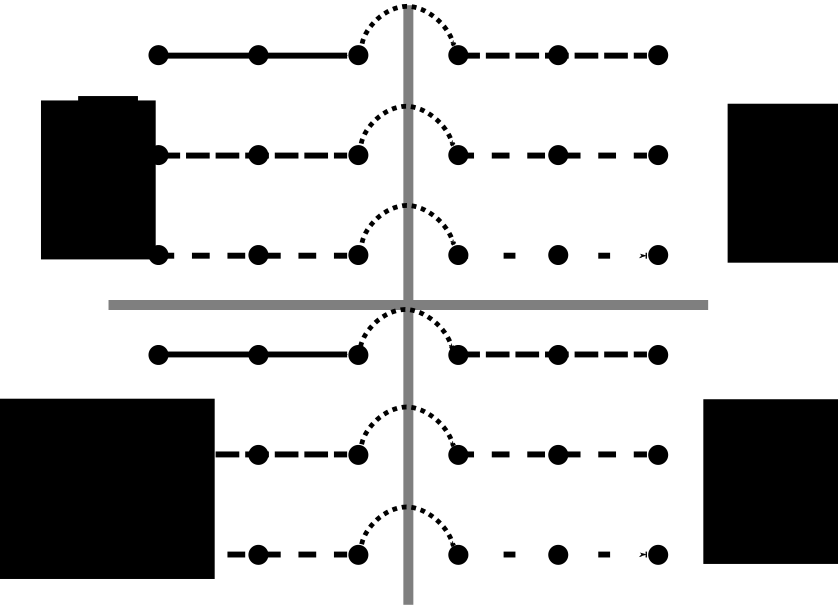
\includegraphics[width=0.95\linewidth]{\imagesdir/sweep_method_forward.png}} \\
            \caption{Метод с использованием неявной схемы. Прямая прогонка.}
            \label{img:sweepforward}
        \end{minipage}
        \hfill
        \begin{minipage}{0.48\linewidth}
            \center{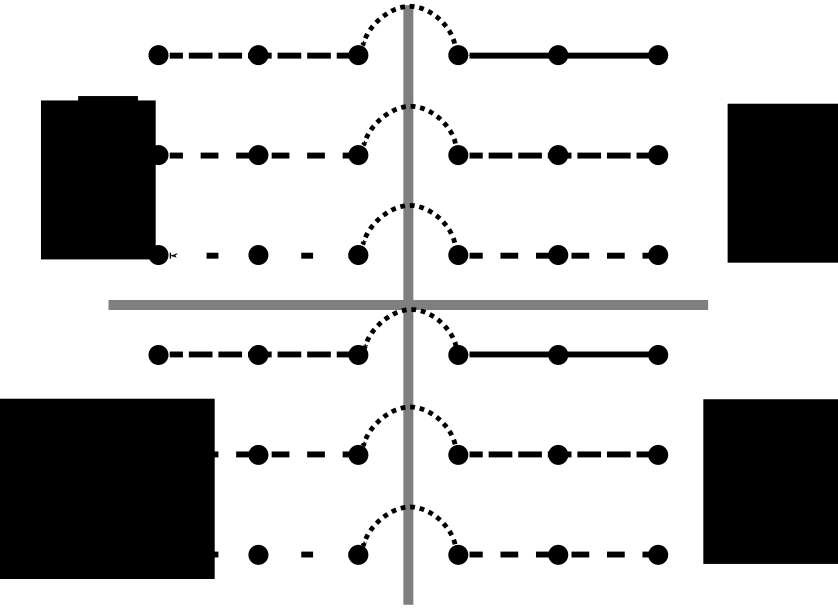
\includegraphics[width=0.95\linewidth]{\imagesdir/sweep_method_backward.png}} \\
            \caption{Метод с использованием неявной схемы. Обратная прогонка.}
            \label{img:sweepbackward}
        \end{minipage}
    \end{center}
\end{figure}

На рис. \ref{img:sweepforward}, \ref{img:sweepbackward} черными точками изображены точки расчетной сетки.
Вертикальная и горизонтальная светло-серые прямые показывают разбиение матрицы поперечного сечения между процессами.
Римские цифры обозначают номера процессов.
Цветные стрелки соответствуют вычислению прогоночных коэффициентов.
Серые стрелки отображают обмены данными между процессами.

Первому расчетному шагу соответствуют стрелки красного цвета.
Для цикла прямой прогонки их выполняют процессы первого столбца матрицы процессов.
Далее эти процессы пересылают посчитанные коэффициенты в граничной точке соседнему справа процессу.
Следующий такт отображен стрелками зеленого цвета, далее следуют синие и коричневые стрелки.
Таким образом, по каждой строке матрицы процессов запускается конвейерная схема параллельных вычислений.

В цикле обратной прогонки конвейерная схема запускается в обратную сторону (соответствие цвета стрелок и порядка выполнения расчетных операций то же).
Пересылке теперь подвергаются расчитанные значения поля.

Отметим две особенности метода.
Во-первых, поскольку цикл обратной прогонки запускается после окончания прямой прогонки по всем строкам расчетной сетки, то необходимо хранить в памяти прогоночные коэффициенты для всех строк, то есть необходима дополнительная матрица для прогоночных коэффициентов того же размера, что и матрица поля.
Во-вторых, для расчета коэффициентов, фигурирующих в разностной системе (\ref{sweep_diff_sys}), необходим обмен значениями поля в граничных областях.

Отметим также, что для высокой эффективности параллельного алгоритма необходимо, чтобы количество строк матрицы поля у отдельного процесса было существенно больше количества процессов в строке матрицы процессов.
Действительно, если число строк у отдельного процесса равно $N_{loc}$, а число процессов в строке матрицы процессов равно $q$ (на рис. \ref{img:sweepforward}, \ref{img:sweepbackward} $N_{loc}=3$, $q=2$), то на цикл прямой прогонки потребуется $N_{loc}+q$ итераций.
Таким образом, верхняя оценка на эффективность имеет вид:
\begin{equation}
    E_n\leqslant\frac{N_{loc}q^2}{q^2(N_{loc} + q)}=\frac{1}{1+q/N_{loc}}.
\end{equation}

В этом соотношении не учтены потери времени на пересылки и синхронизацию процессов. 

    \section{Результаты}

Все реализации были тестированы на корректность на аналитическом решении (свободной дифракции гауссова пучка),
и на консервативность.

Представлены результаты замеров времени работы алгоритма с использованием преобразования Фурье при различных комбинациях параметров, выбранных для анализа их влияния на время работы программы.
Запуск и замеры времени осуществлялись на кластере СКИФ МГУ <<Чебышёв>>.

    \begin{figure}[h!]
        \begin{center}
            \begin{minipage}{0.45\linewidth}
                \center{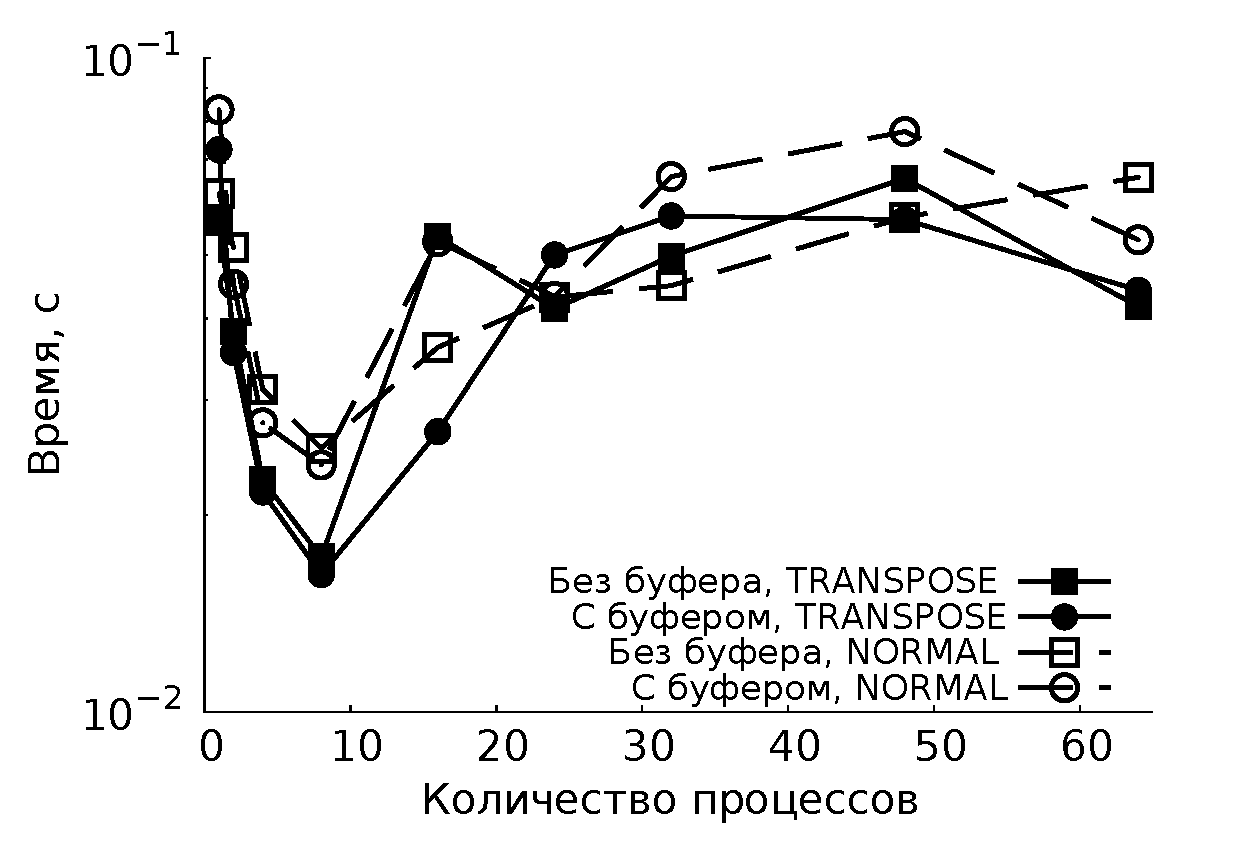
\includegraphics[width=0.95\linewidth]{\graphsdir/Skif/FFTW_compare_N512_nomeasure_all.eps}}
                \caption{Время работы Фурье-алгоритма в зависимости от количества процессов. Размер матрицы 512. Флаг FFTW\_ESTIMATE.}
                \label{gr:Fourier512Nomeasure}
            \end{minipage}
            \hfill
            \begin{minipage}{0.45\linewidth}
                \center{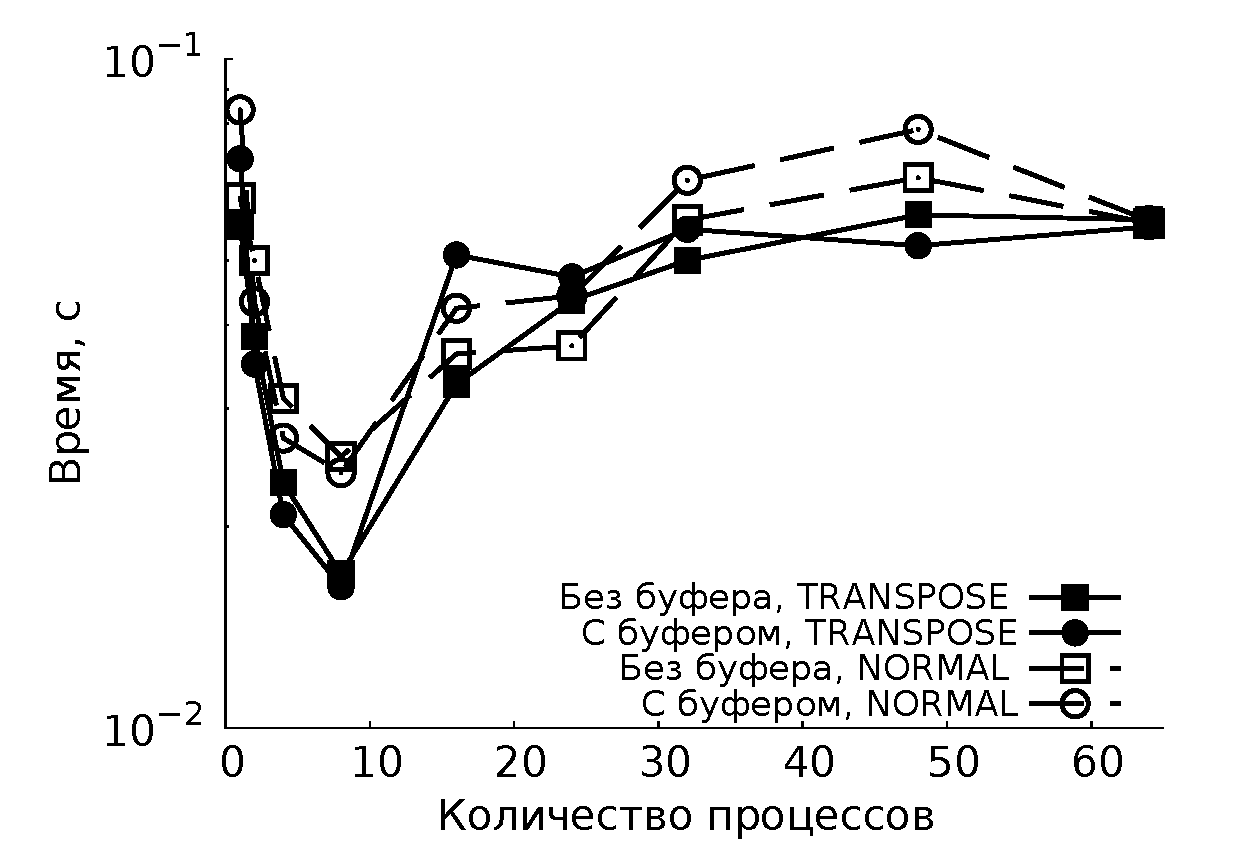
\includegraphics[width=0.95\linewidth]{\graphsdir/Skif/FFTW_compare_N512_measure_all.eps}}
                \caption{Время работы Фурье-алгоритма в зависимости от количества процессов. Размер матрицы 512. Флаг FFTW\_MEASURE.}
                \label{gr:Fourier512Measure}
            \end{minipage}
        \end{center}
    \end{figure}

Из представленных на рис. \ref{gr:Fourier512Nomeasure}, \ref{gr:Fourier512Measure} графиков видно, что использование более 16 процессоров является неэффективным для размера матрицы $N = 512$, так как время работы программы возрастает по сравнению с временем работы программы при тех же параметрах на 8 процессорах.

	\begin{figure}[h!]
		\begin{center}
    		\begin{minipage}{0.48\linewidth}
				\center{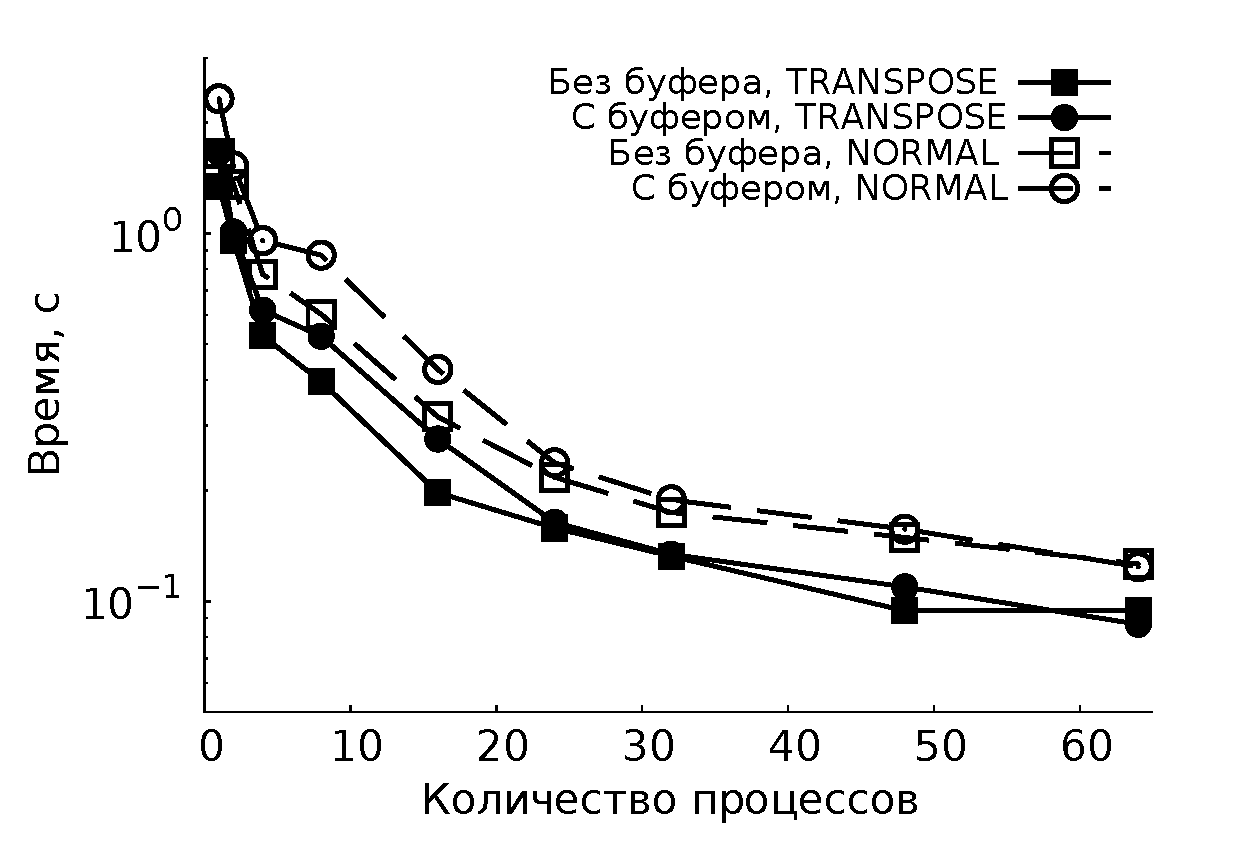
\includegraphics[width=0.95\linewidth]{\graphsdir/Skif/FFTW_compare_N2048_nomeasure_all.eps}}
                \caption{Время работы Фурье-алгоритма в зависимости от количества процессов. Размер матрицы 2048. Флаг FFTW\_ESTIMATE.}
                \label{gr:Fourier2048Nomeasure}
			\end{minipage}
			\hfill
			\begin{minipage}{0.48\linewidth}
				\center{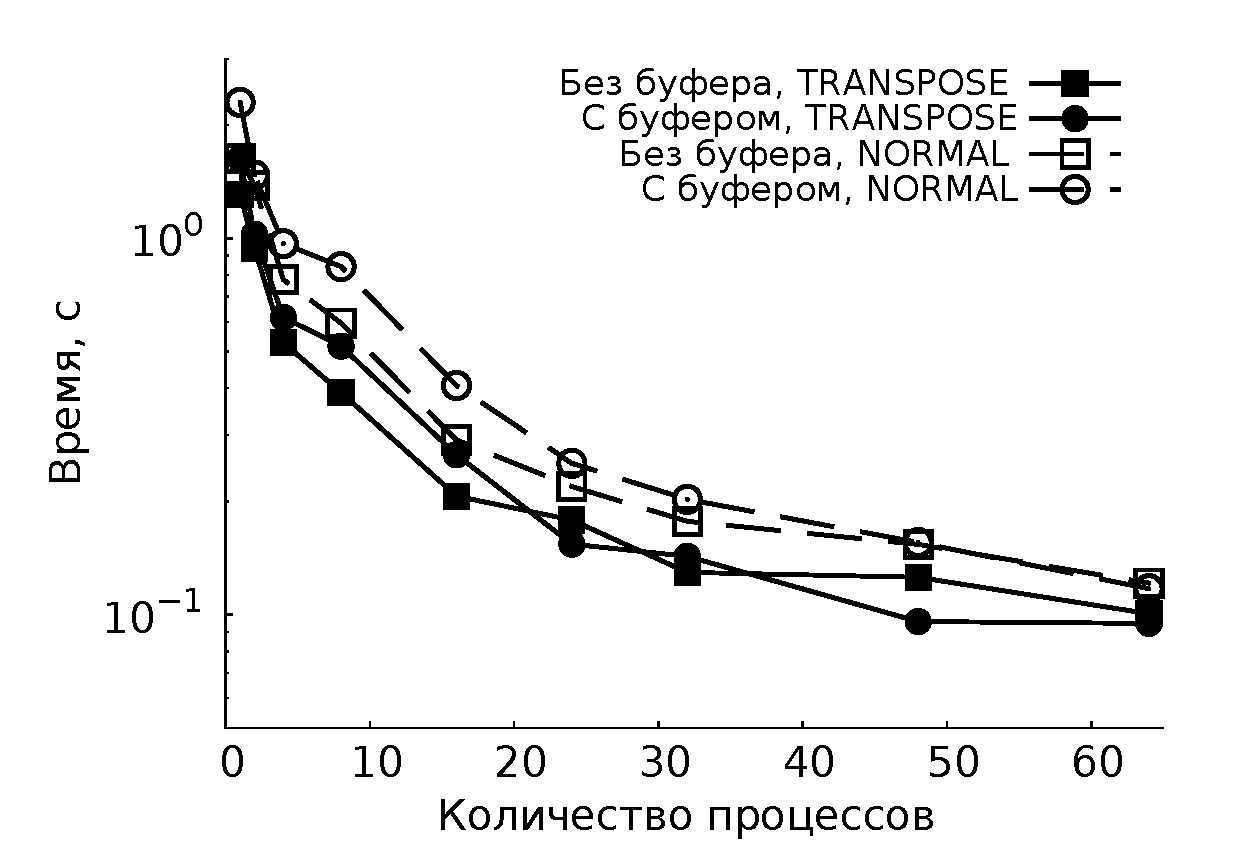
\includegraphics[width=0.95\linewidth]{\graphsdir/Skif/FFTW_compare_N2048_measure_all.eps}}
                \caption{Время работы Фурье-алгоритма в зависимости от количества процессов. Размер матрицы 2048. Флаг FFTW\_MEASURE.}
                \label{gr:Fourier2048Measure}
			\end{minipage}
		\end{center}
	\end{figure}

Для размера матрицы 2048, как видно из рис. \ref{gr:Fourier2048Nomeasure}, \ref{gr:Fourier2048Measure} увеличение числа процессоров от 1 до 16 дает ощутимое уменьшение времени работы программы.
		
	\begin{figure}[h!]
		\begin{center}
			\begin{minipage}{0.45\linewidth}
        		\center{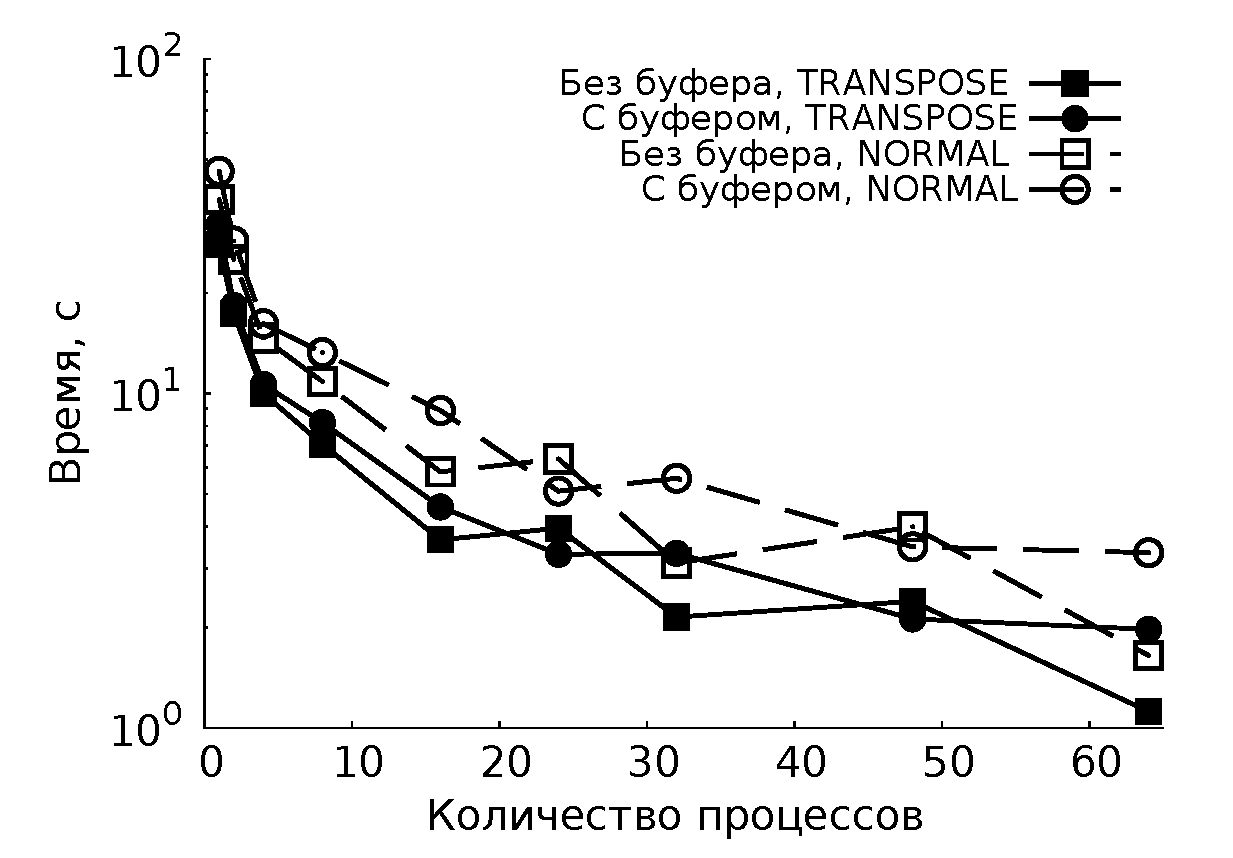
\includegraphics[width=0.95\linewidth]{\graphsdir/Skif/FFTW_compare_N8192_nomeasure_all.eps}}
                \caption{Время работы Фурье-алгоритма в зависимости от количества процессов. Размер матрицы 8192. Флаг FFTW\_ESTIMATE.}
                \label{gr:Fourier8192Nomeasure}
			\end{minipage}
			\hfill
			\begin{minipage}{0.45\linewidth}
				\center{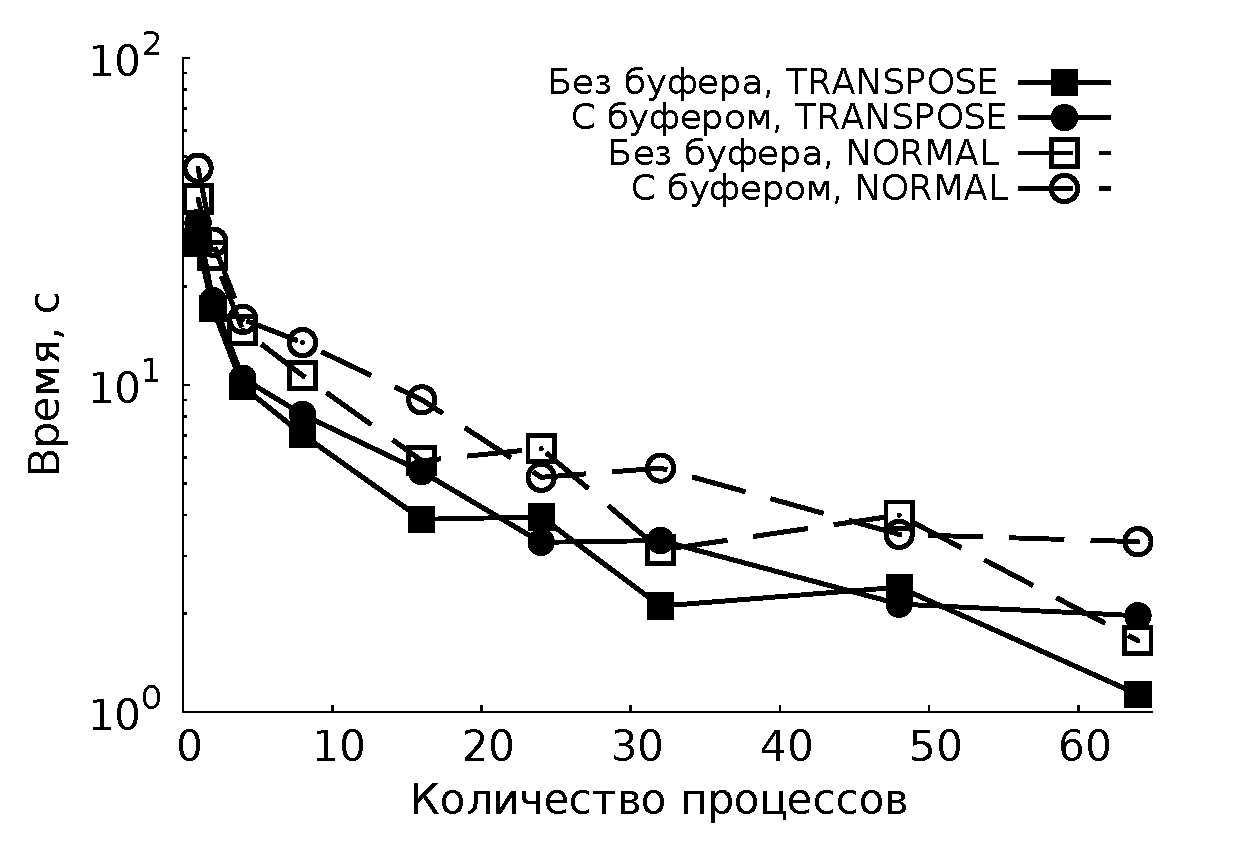
\includegraphics[width=0.95\linewidth]{\graphsdir/Skif/FFTW_compare_N8192_measure_all.eps}}
                \caption{Время работы Фурье-алгоритма в зависимости от количества процессов. Размер матрицы 8192. Флаг FFTW\_MEASURE.}
                \label{gr:Fourier8192Measure}
			\end{minipage}
		\end{center}
	\end{figure}

При использовании матрицы размером 8192 времена работы программы увеличиваются соответственно, что позволяет увидеть более четко различие во временах работы программы при использовании различных комбинаций флагов.

Из графиков на рис. \ref{gr:Fourier512Nomeasure}--\ref{gr:Fourier8192Measure} видно, что использования флага FFTW\_MEASURE не приводит к убыстрению работы алгоритма, что связано прежде всего с малым количеством расчетных узлов.
Кроме того, использование буфера не только не привело к ускорению алгоритма, но, наоборот, несколько затормозило его.
По представленным результатам был сделан вывод, что лучшее враг хорошего. Скорость работы алгоритма с ключом FFTW\_TRANSPOSED\_ORDER, как и ожидалось, оказалась выше, чем с ключом FFTW\_NORMAL\_ORDER.

Было проведено исследование зависимости времени работы алгоритма от используемых ключей компиляции. Результаты представлены в табл. \ref{tab:compilers}.
    \begin{table}[ht]
        \centering
        \begin{tabular}{ | c | c | c | }
            \hline
            Опция		&	$np=8$	&	$np=16$ \\
            \hline
            -O2	(по умолчанию)	&	9.0 с		&	5.0 с \\
            \hline
            -О1		&	9.2 с	 	&	5.3 с \\
            \hline
            -О3		&	8.8 с		&	5.1 с \\
            \hline
            -Оs		&	9.0 с		&	5.2 с \\
            \hline
            -fast	&	8.9 с		&	5.2 с \\
            \hline
        \end{tabular}
        \begin{center}
            \caption{Зависимость времени такта от опций компиляции.}\label{tab:compilers}
        \end{center}
    \end{table}

Таким образом, использование ключей компиляции не дало ощутимого уменьшения времени работы программы.

	\begin{figure}[h!]
		\begin{center}
			\begin{minipage}{0.45\linewidth}
				\center{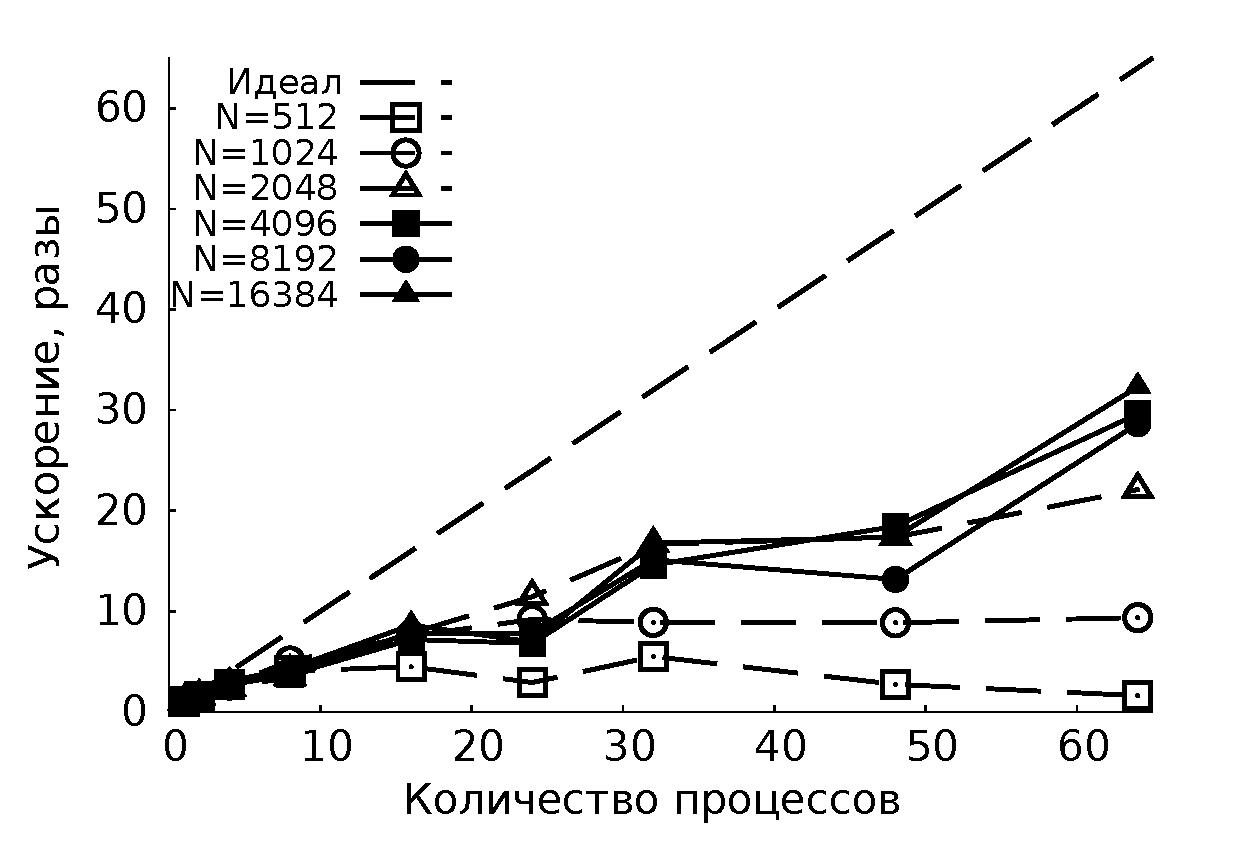
\includegraphics[width=0.95\linewidth]{\graphsdir/Skif/FFTW_acceleration_nosave_all.eps}} \\
                \caption{Ускорение Фурье-алгоритма в зависимости от количества процессов для разных размеров матриц. Сохранение данных в файл не производилось.}
                \label{gr:SpeedupFourierNosave}
			\end{minipage}
			\hfill
			\begin{minipage}{0.45\linewidth}
				\center{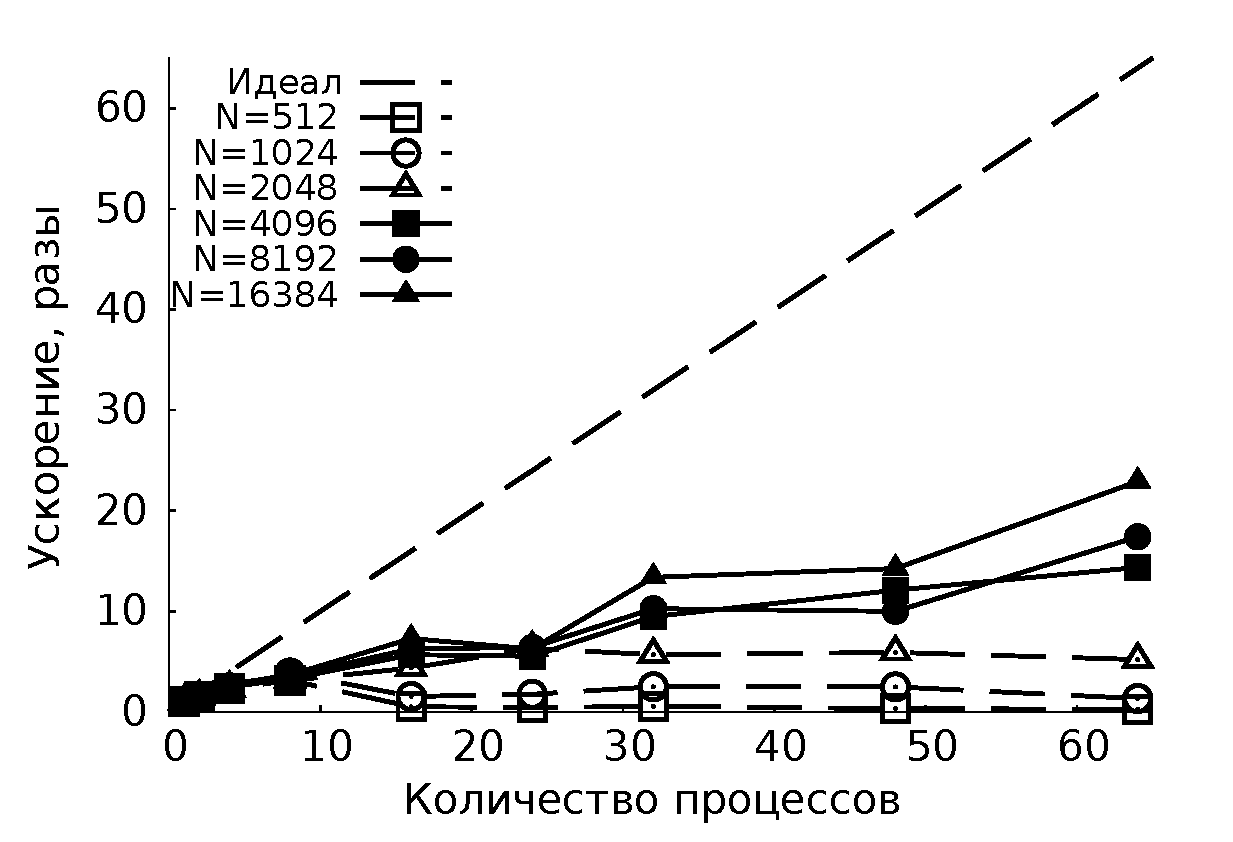
\includegraphics[width=0.95\linewidth]{\graphsdir/Skif/FFTW_acceleration_withsave_all.eps}} \\
                \caption{Ускорение Фурье-алгоритма в зависимости от количества процессов для разных размеров матриц. Сохранение данных в файл производилось на каждом десятом шаге.}
                \label{gr:SpeedupFourierSave}
			\end{minipage}
		\end{center}
	\end{figure}

	\begin{figure}[h!]
		\begin{center}
			\begin{minipage}{0.45\linewidth}
				\center{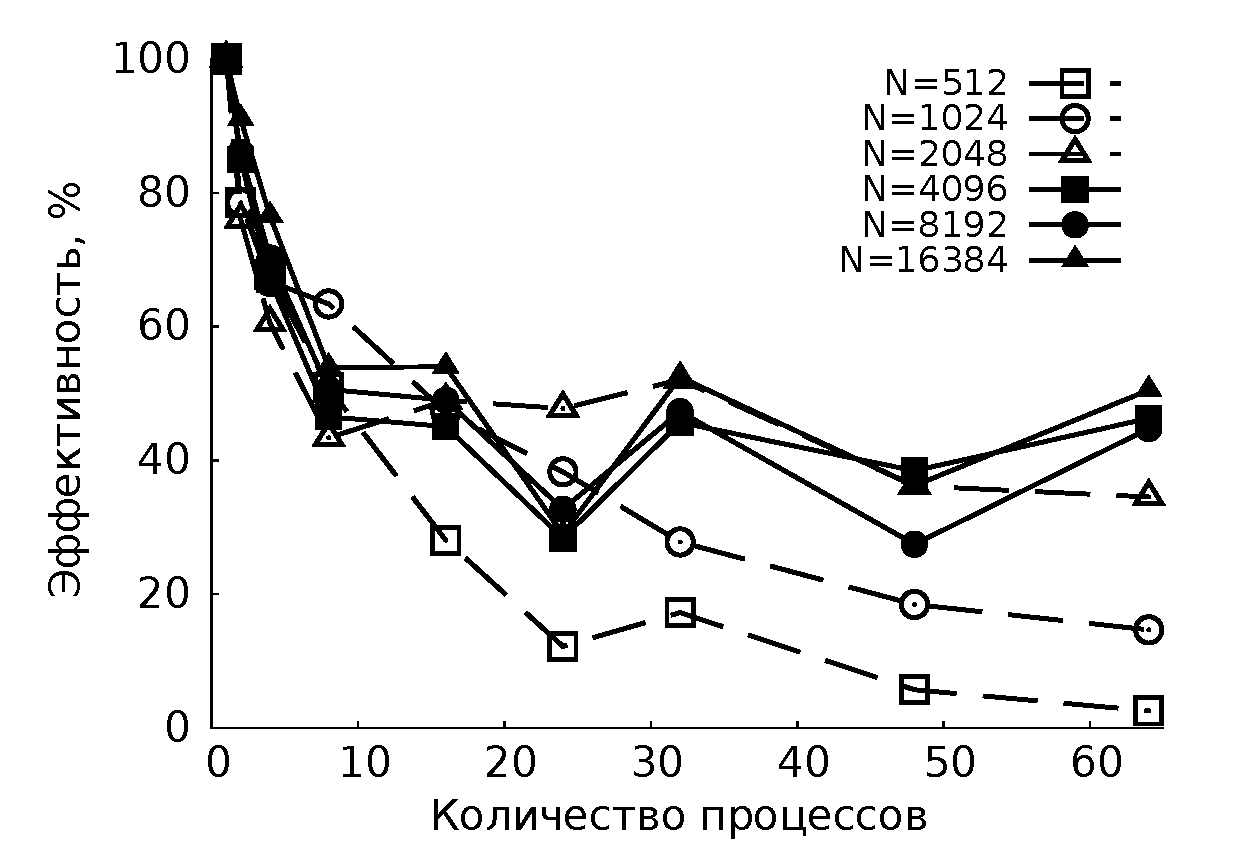
\includegraphics[width=0.95\linewidth]{\graphsdir/Skif/FFTW_efficiency_nosave_all.eps}} \\
                \caption{Эффективность Фурье-алгоритма в зависимости от количества процессов для разных размеров матриц. Сохранение данных в файл не производилось.}
                \label{gr:EfficiencyFourierNosave}
			\end{minipage}
			\hfill
			\begin{minipage}{0.45\linewidth}
				\center{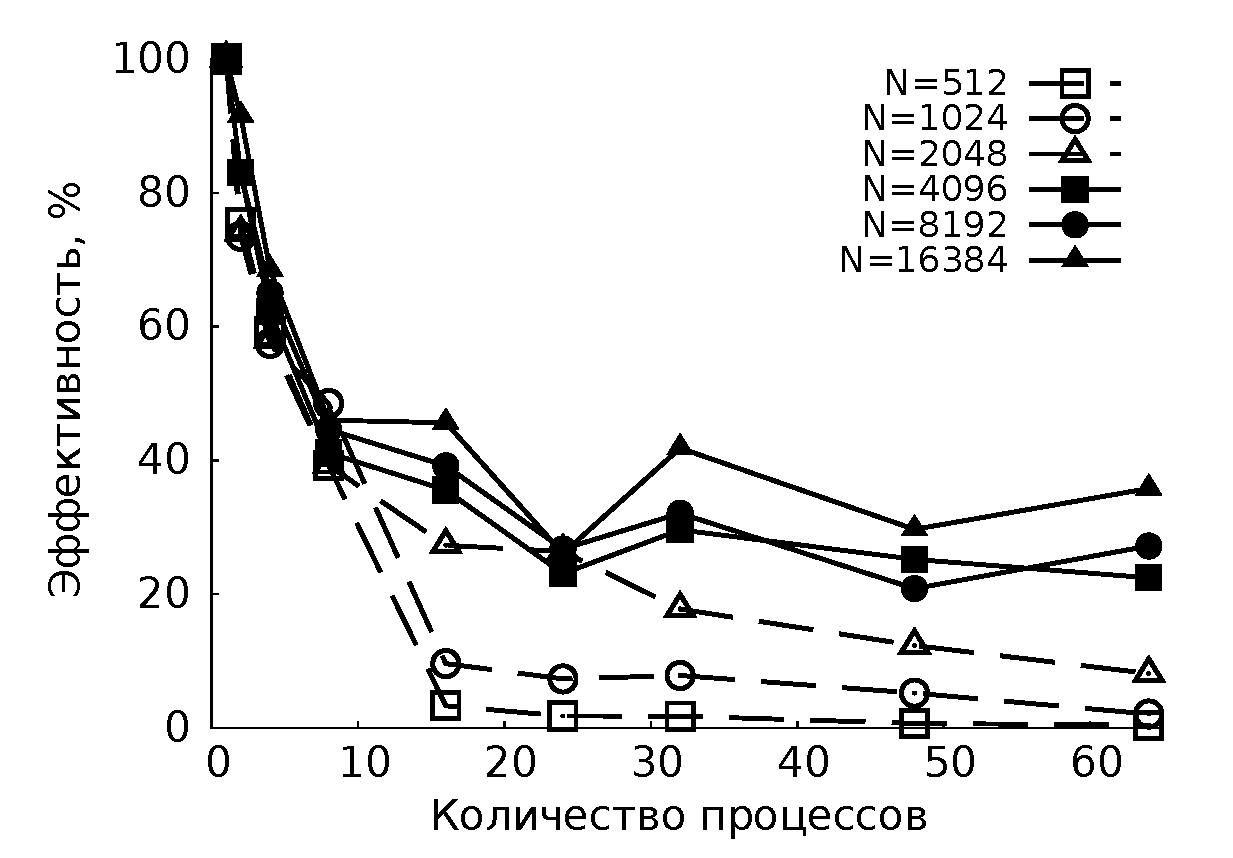
\includegraphics[width=0.95\linewidth]{\graphsdir/Skif/FFTW_efficiency_withsave_all.eps}} \\
                \caption{Эффективность Фурье-алгоритма в зависимости от количества процессов для разных размеров матриц. Сохранение данных в файл производилось на каждом десятом шаге.}
                \label{gr:EfficiencyFourierSave}
			\end{minipage}
		\end{center}
	\end{figure}

Были проведены замеры времени для лучшего набора опций (отсутствие буфера, FFTW\_TRANSPOSED\_ORDER, FFTW\_ESTIMATE).
Замеры проводились без сохранения матрицы в файл и с параллельной записью матрицы в файл на каждом десятом шаге.
Рассчитанные по полученным данным ускорения и эффективности программ представлены на рис. \ref{gr:SpeedupFourierNosave}--\ref{gr:EfficiencyFourierSave}.
Видно, что для размера матрицы поля, не превосходящего $2048\times2048$, использование более 8 процессов нецелесообразно, поскольку не дает прироста скорости.
Эффективность реализации резко падает для размеров матрицы поля $512\times512$ и $1024\times1024$. 
Для больших матриц эффективность остается значительной: около 50\% для случая без сохранения данных и около 30\% для случая с сохранением.
    \begin{figure}[h!]
        \begin{center}
            \begin{minipage}{0.45\linewidth}
                \center{
                    \includegraphics[width=0.95\linewidth]{\graphsdir/Skif/Sweep_acceleration_nosave_all.eps}
                } 
                \caption{Ускорение параллельного алгоритма с неявной схемой. СКИФ МГУ. Сохранение данных в файл не производилось.}
                \label{gr:SweepSpeedupSkifNosave}
			\end{minipage}
			\hfill
			\begin{minipage}{0.45\linewidth}
                \center{
                    \includegraphics[width=0.95\linewidth]{\graphsdir/Skif/Sweep_acceleration_withsave_all.eps}
                }
                \caption{Ускорение параллельного алгоритма с неявной схемой. СКИФ МГУ. Сохранение данных в файл производилось на каждом десятом шаге.}
                \label{gr:SweepSpeedupSkifSave}
			\end{minipage}
		\end{center}
	\end{figure}

    \begin{figure}[h!]
        \begin{center}
            \begin{minipage}{0.45\linewidth}
                \center{
                    \includegraphics[width=0.95\linewidth]{\graphsdir/Skif/Sweep_efficiency_nosave_all.eps}
                }
                \caption{Эффективность параллельного алгоритма с неявной схемой. СКИФ МГУ. Сохранение данных в файл не производилось.}
                \label{gr:SweepEfficiencySkifNosave}
			\end{minipage}
			\hfill
			\begin{minipage}{0.45\linewidth}
				\center{
                    \includegraphics[width=0.95\linewidth]{\graphsdir/Skif/Sweep_efficiency_withsave_all.eps}
                }
                \caption{Эффективность параллельного алгоритма с неявной схемой. СКИФ МГУ. Сохранение данных в файл производилось на каждом десятом шаге.}
                \label{gr:SweepEfficiencySkifSave}
			\end{minipage}
		\end{center}
	\end{figure}

Для алгоритма, использующего неявную схему, проводились замеры времени работы на кластерах СКИФ МГУ <<Чебышёв>> и IBM BlueGene/P.

Результаты замеров времени на СКИФе представлены на рис. \ref{gr:SweepSpeedupSkifNosave}--\ref{gr:SweepEfficiencySkifSave}.
Большие размеры матрицы не позволяли произвести расчет с использованием одного процесса, поэтому нормировка производилась на время работы программы на 4 процессах.

Видно, что при сохранении результатов в ходе работы программы, для матриц размером 512 и 1024 при увеличении числа процессов от 8 до 32 ускорение падает.

Эффективность работы программы при сохранении результатов в ходе работы уменьшается, относительно эффективности работы программы не сохраняющей результаты расчетов в файлы. Увеличение числа процессов эффективно при размере матрицы более 1024, если происходит сохранение результатов.
	\begin{figure}[h!]
		\begin{center}
			\begin{minipage}{0.45\linewidth}
				\center{
                    \includegraphics[width=0.95\linewidth]{\graphsdir/Bluegene/Sweep_acceleration_nosave_all.eps}
                }
                \caption{Ускорение параллельного алгоритма с неявной схемой. BlueGene/P. Сохранение данных в файл не производилось.}
                \label{gr:SweepSpeedupBluegeneNosave}
			\end{minipage}
			\hfill
			\begin{minipage}{0.45\linewidth}
                \center{
                    \includegraphics[width=0.95\linewidth]{\graphsdir/Bluegene/Sweep_acceleration_withsave_all.eps}
                }
                \caption{Ускорение параллельного алгоритма с неявной схемой. BlueGene/P. Сохранение данных в файл производилось на каждом десятом шаге.}
                \label{gr:SweepSpeedupBluegeneSave}
			\end{minipage}
		\end{center}
	\end{figure}
    \begin{figure}[h!]
        \begin{center}
            \begin{minipage}{0.45\linewidth}
                \center{
                    \includegraphics[width=0.95\linewidth]{\graphsdir/Bluegene/Sweep_efficiency_nosave_all.eps}
                }
                \caption{Эффективность параллельного алгоритма с неявной схемой. BlueGene/P. Сохранение данных в файл не производилось.}
                \label{gr:SweepEfficiencyBluegeneNosave}
            \end{minipage}
            \hfill
            \begin{minipage}{0.45\linewidth}
                \center{
                    \includegraphics[width=0.95\linewidth]{\graphsdir/Bluegene/Sweep_efficiency_withsave_all.eps}
                }
                \caption{Эффективность параллельного алгоритма с неявной схемой. BlueGene/P. Сохранение данных в файл производилось на каждом десятом шаге.}
                \label{gr:SweepEfficiencyBluegeneSave}
            \end{minipage}
        \end{center}
    \end{figure}
    
Результаты замеров времени работы алгоритма с использованием неявной схемы на кластере IBM Bluegene/P приведены на рис. \ref{gr:SweepSpeedupBluegeneNosave}--\ref{gr:SweepEfficiencyBluegeneSave}.

Большие размеры матрицы не позволяли произвести расчет с использованием одного процесса, поэтому нормировка производилась на время работы программы на 8 процессах. Видно стабильное линейное увеличение ускорения работы программы при увеличении числа процессоров уже для сравнительно небольших матриц.
Эффективность реализации близка к единице.
Таким образом, при работе на IBM Bluegene/P, увеличение числа процессов, на которых запускается программа,
эффективно. Однако, время выполнения шага интегрирования на IBM Bluegene/P существенно больше, чем на СКИФе, что связано с существенно более слабыми процессорами. 


    \vspace{1em}
\noindent \textbf{5. Выводы.}
\vspace{0.5em}

В рамках работы было проведено исследование различных алгоритмов решения нелинейного уравнения квазиоптики (нелинейного уравнения Шредингера).
Рассматривались методы с использованием разностных схем и метод с применением преобразования Фурье.

Тестовые эксперименты показали, что при использовании схемы предиктор-корректор (Рунге-Кутта 4-го порядка)
из-за наличия поперечных координат и участия в уравнении производной по ним необходимо
использовать слишком маленький шаг по координате z для получения устойчивого решения.
Таким образом, эту схему имеет смысл использовать в расчётах, где величина шага уже лимитирована
другими особенностями поставленной задачи. Также следует отметить, что для реализации этого алгоритма
необходимо держать в памяти 3 дополнительные матрицы равные по размеру основной,
а на каждом шаге необходимо 4 раза обмениваться граничными значениями локальных блоков матрицы.

В случае применения неявной консервативной схемы, устойчивой при любом шаге интегрирования,
шаг необходимо выбирать основываясь на эмпирических физических оценках.
Кроме того, для реализации этого алгоритма требуется только одна дополнительная матрица,
равная основной (она используется для хранения коэффициентов метода прогонки).
Алгоритм показал отличную масштабируемость на кластере IBM Bluegene/P,
которая не сильно пострадала даже в случае периодического сохранения данных вычислений на диск.
Это объясняется небольшой тактовой частотой процессоров при наличии быстрой сети и применении MPI Parallel I/O.

При использовании Фурье-метода можно обойтись без использования дополнительной матрицы,
тем самым по сравнению с методом Рунге-Кутта увеличить размер расчётной сетки в 2 раза
по каждой координате при использовании того же количества памяти.
Из-за более сложной организации пересылок при расчёте параллельного Фурье-преобразования
по сравнению с остальными алгоритмами его масштабируемость ниже.
Также наблюдается провал в производительности при небольших размерах матриц.
Однако скорость вычислений для этого метода больше, по крайней мере при использовании до 64 процессов,
что для применения на СКИФ МГУ <<Чебышёв>> делает его более удачным.

Таким образом, нельзя чётко сказать, какой метод является лучше в общем случае.
В случае, если задача не накладывает каких-то особых ограничений, лучше использовать Фурье-метод.
Если же имеется возможность использовать для расчёта очень большое число процессоров,
то целесообразно применения метода с неявной разностной схемой. Также этот метод будет применим
для задач с неравномерной сеткой по поперечному сечению, так как для них нет алгоритма
быстрого преобразования Фурье и метод с его использованием теряет свою актуальность.

Коллектив авторов выражает благодарность администрации кластеров СКИФ <<Чебышёв>> НИВЦ МГУ и IBM Bluegene/P ВМиК МГУ
за предоставленное процессорное время для проведения тестирования алгоритмов.


    % Examples:
    % \textit{Бахвалов Н.С., Жидков Н.П., Кобельков Г.М.} Численные методы. М.: Наука, 1987.
    % Вычислительные методы линейной алгебры. Тр. I Всесоюзной конференции. Новосибирск: ВЦ СО АН СССР, 1969. 
    % \textit{Зельдович Я.Б.} К теории распространения детонации в газообразных системах // Журн. экспер. и теор. физ. 1940. 10, вып. 5. 542-568. 
    \begin{thebibliography}{99}
        \bibitem{KandidovShlenovKosarevaReview2009}%
        \textit{Кандидов В.П., Шлёнов С.А., Косарева О.Г.}
        Филаментация мощного фемтосекундного лазерного излучения.
        Квантовая электроника, 39, 3, 2009.

        \bibitem{LadaginStarikov1998}%
        \textit{Ладагин В.К., Стариков Ф.А.}
        Численное решение квазиоптического уравнения для поперечной корреляционной функции поля излучения.
        Математическое моделирование, 10, 8, 1998.

        \bibitem{Agrawal2001}%
        \textit{Agrawal G.P.}
        Applications of Nonlinear Fiber Optics (3rd edition).
        Elsevier Science, 2001.

        \bibitem{Mahankov1983}%
        \textit{Маханьков В.Г.}
        Солитоны и численный эксперимент.
        Физика элементраных частиц и атомного ядра, 14, 1, 1983.

        \bibitem{VitkovskiyFedoruk2008}%
        \textit{Витковский В.Э., Федорук М.П.}
        Численное исследование свойств решений нелинейного уравнения Шредингера при распространении лазерных импульсов в световодах.
        Вычислительные технологии, 13, 6, 2008.

        \bibitem{Kadomcev1997}%
        \textit{Кадомцев Б.Б., Кадомцев М.Б.}
        Конденсаты Бозе-Эйнштейна.
        УФН, 167, 6, 1997.

        \bibitem{Belyaeva2005}%
        \textit{Беляева Л.Т. и др.}
        Динамика солитонов в модели нелинейного уравнения Шредингера с внешним гармоническим потенциалом.
        Квантовая Электроника, 35, 9, 2005.

        \bibitem{Kartvenko1993}%
        \textit{Картавенко В.Г.}
        Линейные и нелинейные возбуждения ядерной плотности.
        Физика элементарных частиц и атомного ядра, 24, 6, 1993.

        \bibitem{Zeytunyan1995}%
        \textit{Зейтунян Р.Х.}
        Нелинейные длинные волны на поверхности воды.
        Успехи Физических Наук, 165, 12, 1995.

        \bibitem{RK_Rado_Lobatto}%
        \textit{Хайрер Э., Ваннер Г.}
        Решение обыкновенных дифференциальных уравнений. Жёсткие и дифференциально-алгебраические задачи.
        М., Мир, 1999, 685.

        \bibitem{RK_Parallel_Houwen_2001}%
        \textit{Houwen P.J., Sommeijer B.P.} Parallel ODE solver.
        // Proceedings of the International Conference on Supercomputing.
        2001, 71--81.

        \bibitem{RK_Parallel_Jackson_2001}%
        \textit{Jackson K.R., Norsett S.P.}
        The potential for parallelism in Runge-Kutta methods.Part 1: R-K formulas in standard form.
        SIAM J.Numer. Anal. 32, 2001, 49--82.

        \bibitem{FFTW}%
        http://fftw.org

        \bibitem{FFTW2_Generator_99}% This paper describes the codelet generator introduced in FFTW 2
        \textit{Matteo Frigo.} A fast Fourier transform compiler
        // Proc. 1999 ACM SIGPLAN Conf. on Programming Language Design and Implementation.
        1999. Vol. 34, num. 5, 169--180.

        \bibitem{FFTW1_98}% This was the main paper describing FFTW 1
        \textit{Matteo Frigo, Steven G. Johnson.} FFTW: An adaptive software architecture for the FFT
        // Proc. 1998 IEEE Intl. Conf. Acoustics Speech and Signal Processing.
        1998. Vol. 3, 1381--1384.

        \bibitem{Kalitkin}%
        \textit{Калиткин Н.Н.}
        Численные методы.
        М., Наука, 1978.

        \bibitem{SweepScheme}%
        \textit{V.P. Kandidov, V.Yu. Fedorov.}
        Properties of self-focusing in elliptic beams.
        Quantum Electronics, 34, 12, 2004.
    \end{thebibliography}

\end{document}
